\documentclass[11pt]{article}

\usepackage[a4paper,margin=22mm]{geometry}
\usepackage{amsmath}
\usepackage{graphicx}
\usepackage{booktabs}
\usepackage{array}
\usepackage{xcolor}
\usepackage{enumitem}
\usepackage{titlesec}
\usepackage{fancyhdr}
\usepackage{longtable}
\usepackage{needspace}
\usepackage[hidelinks]{hyperref}

\definecolor{ink}{HTML}{222222}
\definecolor{accent}{HTML}{0072B2}
\definecolor{ok}{HTML}{009E73}
\definecolor{soft2}{HTML}{8C8C8C}

\color{ink}
\titleformat{\section}{\Large\bfseries\color{accent}}{\thesection}{0.6em}{}
\titleformat{\subsection}{\normalsize\bfseries\color{ink}}{}{0em}{}
\setlist{itemsep=2pt,topsep=3pt,parsep=0pt}
\renewcommand{\arraystretch}{1.18}
\setlength{\LTpre}{4pt}\setlength{\LTpost}{8pt}

\pagestyle{fancy}\fancyhf{}
\lhead{\small\color{accent}OptiComp2}
\rhead{\small Verification register}
\cfoot{\small\thepage}
\renewcommand{\headrulewidth}{0.4pt}

\newcommand{\code}[1]{\texttt{\small #1}}

\begin{document}

% ---- title ----
\thispagestyle{empty}
\vspace*{2.2cm}
\begin{center}
{\Huge\bfseries\color{accent} OptiComp2}\\[6pt]
{\LARGE\bfseries Verification register and test report}\\[16pt]
{\large Every automated test of the instrument-control software, with coverage figures}\\[26pt]
{\large Haoxiang Zhang}\\[6pt]
{\normalsize August 2026 \quad$\cdot$\quad 149 tests \quad$\cdot$\quad 9 modules \quad$\cdot$\quad 31 test classes}
\end{center}
\vfill
\noindent\small This report lists every automated test in OptiComp2, grouped by module and by what it
verifies, together with the coverage figures. The whole suite runs without any hardware --- against a
fake serial port and a fake spectrometer DLL --- so it can be run on a workstation and on the
instrument PC alike. It is the executable specification of the safety and correctness properties
described in the change list.
\newpage

\tableofcontents
\newpage

% ---- 1 summary ----
\section{Summary}

\begin{center}
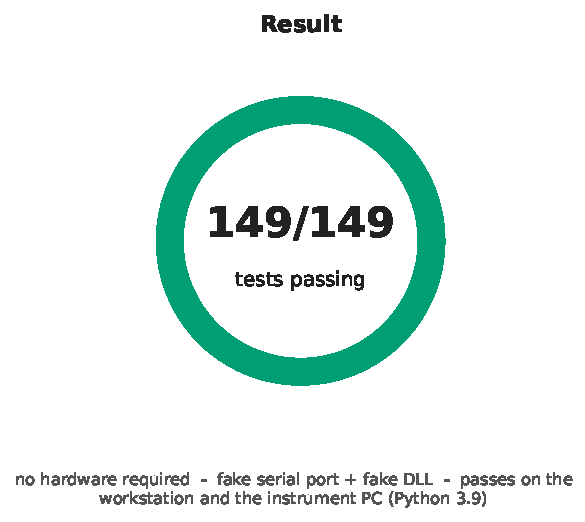
\includegraphics[width=0.52\linewidth]{figures/vfig_pass.pdf}
\end{center}

\noindent The suite comprises \textbf{149 tests} in 31 classes across 9 modules, and all pass. Run it
with:
\begin{quote}\code{py -m unittest discover -s tests}\end{quote}
Every test uses in-memory fakes (a scripted serial port, a fake \code{BWTEKUSB.dll}, a demo bus and
spectrometer), so no instrument, lamp or motion is involved and the suite is deterministic and safe to
run anywhere. Fault injection (swallowed commands, truncated replies, a hung DLL, a corrupt manifest,
an operator-absent pause) is used to exercise the recovery and abort paths that matter most on the
real instrument.

\section{Coverage by theme}

\begin{center}
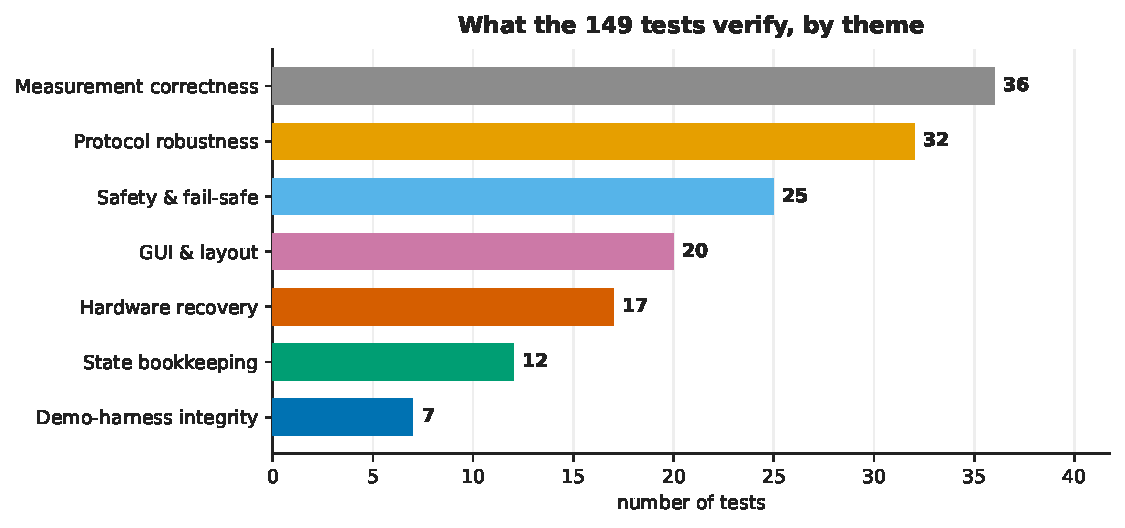
\includegraphics[width=0.96\linewidth]{figures/vfig_theme.pdf}
\end{center}

\noindent The tests are grouped below by the property they establish:
\begin{itemize}
\item \textbf{Measurement correctness (36)} --- the reflectance relation, dark matching, saturation and
invalid-wavelength masking, the Fresnel/BK7 standards, the scan gatekeeper, manifest bookkeeping and
integration-time calibration.
\item \textbf{Protocol robustness (32)} --- reply decoding, swallowed-command resend, stray/truncated
replies, timeouts, corrective moves and the mechanical-timeout policy on the Elliptec bus.
\item \textbf{Safety \& fail-safe (25)} --- the shutter is closed on any error or abort, the fibre arm
is protected from homing, soft limits hold, auto integration time aborts on no light, and the
state gate blocks motion after an anomaly.
\item \textbf{GUI \& layout (20)} --- the theme and widgets, the end-to-end demo tour, the feature-
parity reference and the layout audit at two window sizes.
\item \textbf{Hardware recovery (17)} --- the spectrometer reopen / USB-restart ladder and the
monitor/cycle tools recovering from an injected read failure.
\item \textbf{State bookkeeping (12)} --- the motor-state record: round-trip, wrap-around comparison,
settling tolerance and corrupt-record handling.
\item \textbf{Demo-harness integrity (7)} --- the fakes never touch real hardware and reproduce
realistic, seeded spectra.
\end{itemize}

\section{Coverage by module}

\begin{center}
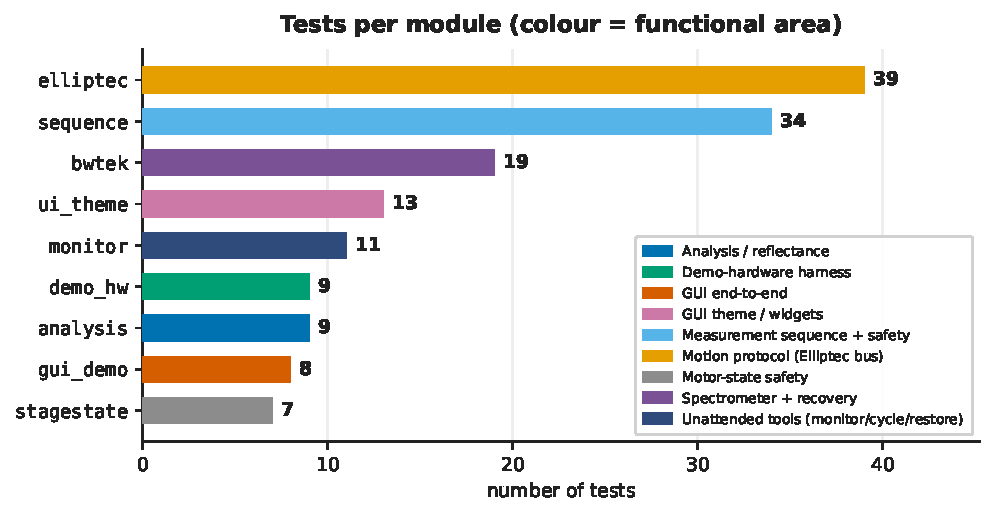
\includegraphics[width=0.96\linewidth]{figures/vfig_module.pdf}
\end{center}

\begin{center}\small
\begin{tabular}{@{}>{\ttfamily}l l r@{}}
\toprule
\normalfont\textbf{Module} & \textbf{Functional area} & \textbf{Tests} \\
\midrule
test\_elliptec.py & Motion protocol (Elliptec bus) & 39 \\
test\_sequence.py & Measurement sequence and safety & 34 \\
test\_bwtek.py & Spectrometer and recovery & 19 \\
test\_ui\_theme.py & GUI theme and widgets & 13 \\
test\_monitor.py & Unattended tools (monitor / cycle / restore) & 11 \\
test\_analysis.py & Analysis and reflectance & 9 \\
test\_demo\_hw.py & Demo-hardware harness & 9 \\
test\_gui\_demo.py & GUI end-to-end (demo hardware) & 8 \\
test\_stagestate.py & Motor-state safety & 7 \\
\midrule
\normalfont\textbf{Total} & & \textbf{149} \\
\bottomrule
\end{tabular}
\end{center}

\section{Methodology}
\begin{itemize}
\item \textbf{No hardware.} A scripted serial port answers Elliptec queries from a table; a fake DLL
returns canned frames and error codes; a demo bus and spectrometer drive the GUI. The production code
path is exercised unchanged --- only the lowest-level back-end is substituted.
\item \textbf{Fault injection.} Tests force the failure modes seen on the instrument: a swallowed
\code{ma}, a reply truncated by the read timeout, a stray reply from another module, a mechanical
timeout (\code{GS02}), a hung DLL (read $-99$), a corrupt manifest and an operator-absent pause --- and
assert the resend, discard, abort or recovery that must follow.
\item \textbf{Safety assertions.} The shutter-closing, protected-home and soft-limit properties are
asserted directly (for example, an error raised with the shutter open must leave it closed).
\item \textbf{GUI.} The demo tour drives the whole workflow in the Tk loop and a layout audit checks
that no widget is clipped at 1280$\times$820 or 1100$\times$720.
\item \textbf{Both platforms.} The suite passes on a workstation and on the instrument PC
(Python~3.9, \code{py -m unittest discover -s tests}), with no third-party test runner.
\end{itemize}

\newpage
\section{Full test register}
\small Each test is listed with its one-line purpose (from the test's own comment, or its name where it
is self-describing). Test names are the exact method names, for traceability.
\normalsize

\subsection{Motion protocol (Elliptec bus) \hfill \normalfont\small\color{soft2}\texttt{test\_elliptec.py} $\cdot$ 39 tests}
\needspace{4\baselineskip}
\par\smallskip \textbf{CodecTests}\par\nopagebreak\smallskip
\begin{longtable}{@{}>{\ttfamily\scriptsize\raggedright\arraybackslash}p{0.40\linewidth} >{\footnotesize\raggedright\arraybackslash}p{0.555\linewidth}@{}}
test\_\allowbreak{}hex32\_\allowbreak{}roundtrip & Hex32 roundtrip \\
test\_\allowbreak{}info\_\allowbreak{}decode\_\allowbreak{}full\_\allowbreak{}serial & Info decode full serial \\
test\_\allowbreak{}gs\_\allowbreak{}po\_\allowbreak{}decode & Gs po decode \\
\end{longtable}
\needspace{4\baselineskip}
\par\smallskip \textbf{BusTests}\par\nopagebreak\smallskip
\begin{longtable}{@{}>{\ttfamily\scriptsize\raggedright\arraybackslash}p{0.40\linewidth} >{\footnotesize\raggedright\arraybackslash}p{0.555\linewidth}@{}}
test\_\allowbreak{}query\_\allowbreak{}timeout\_\allowbreak{}raises & Query timeout raises \\
test\_\allowbreak{}info\_\allowbreak{}and\_\allowbreak{}position & Info and position \\
test\_\allowbreak{}move\_\allowbreak{}waits\_\allowbreak{}while\_\allowbreak{}busy\_\allowbreak{}then\_\allowbreak{}reads\_\allowbreak{}position & Move waits while busy then reads position \\
test\_\allowbreak{}swallowed\_\allowbreak{}command\_\allowbreak{}is\_\allowbreak{}resent & Real-bus case 2026-08-25: no reply, no motion, GS00 -$>$ resend; second attempt works \\
test\_\allowbreak{}swallowed\_\allowbreak{}command\_\allowbreak{}gives\_\allowbreak{}up\_\allowbreak{}after\_\allowbreak{}attempts & Swallowed command gives up after attempts \\
test\_\allowbreak{}wrong\_\allowbreak{}final\_\allowbreak{}position\_\allowbreak{}raises & Wrong final position raises \\
test\_\allowbreak{}small\_\allowbreak{}residual\_\allowbreak{}triggers\_\allowbreak{}corrective\_\allowbreak{}move & Real-bus case: ELL18 stopped 42 pulses short after a long move; a second `ma` fixes it \\
test\_\allowbreak{}persistent\_\allowbreak{}small\_\allowbreak{}residual\_\allowbreak{}is\_\allowbreak{}accepted\_\allowbreak{}with\_\allowbreak{}warning & Persistent small residual is accepted with warning \\
test\_\allowbreak{}relative\_\allowbreak{}move\_\allowbreak{}correction\_\allowbreak{}uses\_\allowbreak{}absolute\_\allowbreak{}target & Relative move correction uses absolute target \\
test\_\allowbreak{}lost\_\allowbreak{}reply\_\allowbreak{}but\_\allowbreak{}move\_\allowbreak{}completed & Lost reply but move completed \\
test\_\allowbreak{}motion\_\allowbreak{}uses\_\allowbreak{}long\_\allowbreak{}timeout\_\allowbreak{}and\_\allowbreak{}restores & Motion uses long timeout and restores \\
test\_\allowbreak{}deferred\_\allowbreak{}po\_\allowbreak{}arrives\_\allowbreak{}during\_\allowbreak{}gs\_\allowbreak{}poll & Real-bus case: ELL18 silent while moving, completion PO lands in the `gs` read window \\
test\_\allowbreak{}truncated\_\allowbreak{}late\_\allowbreak{}po\_\allowbreak{}fragment\_\allowbreak{}is\_\allowbreak{}discarded & Real-bus case 2026-08-25 21:53: the completion PO of module 2 arrived while the input buffer \\
test\_\allowbreak{}stray\_\allowbreak{}reply\_\allowbreak{}from\_\allowbreak{}other\_\allowbreak{}module\_\allowbreak{}is\_\allowbreak{}discarded & Stray reply from other module is discarded \\
test\_\allowbreak{}only\_\allowbreak{}stray\_\allowbreak{}replies\_\allowbreak{}raises & Only stray replies raises \\
test\_\allowbreak{}mechanical\_\allowbreak{}timeout\_\allowbreak{}retried\_\allowbreak{}once & Mechanical timeout retried once \\
test\_\allowbreak{}sensor\_\allowbreak{}error\_\allowbreak{}at\_\allowbreak{}target\_\allowbreak{}is\_\allowbreak{}accepted & Real-bus case: GS0A after a long move, but gp shows the stage at the target \\
test\_\allowbreak{}sensor\_\allowbreak{}error\_\allowbreak{}off\_\allowbreak{}target\_\allowbreak{}raises & Sensor error off target raises \\
test\_\allowbreak{}mechanical\_\allowbreak{}timeout\_\allowbreak{}twice\_\allowbreak{}raises & Mechanical timeout twice raises \\
test\_\allowbreak{}mechanical\_\allowbreak{}timeout\_\allowbreak{}recovers\_\allowbreak{}within\_\allowbreak{}default\_\allowbreak{}retries & Two GS02s then a good move: the default retry budget (3) rides out a couple of stalls \\
test\_\allowbreak{}shutter\_\allowbreak{}already\_\allowbreak{}open\_\allowbreak{}is\_\allowbreak{}accepted & Shutter already open is accepted \\
test\_\allowbreak{}shutter\_\allowbreak{}swallowed\_\allowbreak{}fw\_\allowbreak{}is\_\allowbreak{}resent & Shutter swallowed fw is resent \\
test\_\allowbreak{}move\_\allowbreak{}error\_\allowbreak{}status\_\allowbreak{}raises & Move error status raises \\
test\_\allowbreak{}wrong\_\allowbreak{}address\_\allowbreak{}reply\_\allowbreak{}raises & Wrong address reply raises \\
test\_\allowbreak{}rotation\_\allowbreak{}stage\_\allowbreak{}degrees & Rotation stage degrees \\
\end{longtable}
\needspace{4\baselineskip}
\par\smallskip \textbf{ReplyIntegrityTests} \;{\small\itshape 2026-08-26 review: partial lines and out-of-order kinds must never be taken as answers.}\par\nopagebreak\smallskip
\begin{longtable}{@{}>{\ttfamily\scriptsize\raggedright\arraybackslash}p{0.40\linewidth} >{\footnotesize\raggedright\arraybackslash}p{0.555\linewidth}@{}}
test\_\allowbreak{}truncated\_\allowbreak{}payload\_\allowbreak{}is\_\allowbreak{}an\_\allowbreak{}error & Truncated payload is an error \\
test\_\allowbreak{}unterminated\_\allowbreak{}fragment\_\allowbreak{}is\_\allowbreak{}discarded & Readline() returned a fragment cut by the timeout, the real line follows \\
test\_\allowbreak{}complete\_\allowbreak{}line\_\allowbreak{}without\_\allowbreak{}terminator\_\allowbreak{}is\_\allowbreak{}not\_\allowbreak{}trusted & Complete line without terminator is not trusted \\
test\_\allowbreak{}late\_\allowbreak{}po\_\allowbreak{}before\_\allowbreak{}gs\_\allowbreak{}answer\_\allowbreak{}is\_\allowbreak{}skipped & A completion PO arrives just before the answer to our gs \\
test\_\allowbreak{}home\_\allowbreak{}is\_\allowbreak{}never\_\allowbreak{}repeated\_\allowbreak{}after\_\allowbreak{}mechanical\_\allowbreak{}timeout & Home is never repeated after mechanical timeout \\
test\_\allowbreak{}relative\_\allowbreak{}move\_\allowbreak{}retries\_\allowbreak{}as\_\allowbreak{}absolute & Relative move retries as absolute \\
\end{longtable}
\needspace{4\baselineskip}
\par\smallskip \textbf{PollRobustnessTests}\par\nopagebreak\smallskip
\begin{longtable}{@{}>{\ttfamily\scriptsize\raggedright\arraybackslash}p{0.40\linewidth} >{\footnotesize\raggedright\arraybackslash}p{0.555\linewidth}@{}}
test\_\allowbreak{}stray\_\allowbreak{}line\_\allowbreak{}burst\_\allowbreak{}during\_\allowbreak{}gs\_\allowbreak{}poll\_\allowbreak{}is\_\allowbreak{}not\_\allowbreak{}fatal & A stray-line burst makes query() raise a generic ElliptecError (not ReplyTimeout); \\
\end{longtable}
\needspace{4\baselineskip}
\par\smallskip \textbf{ProtectedHomeTests}\par\nopagebreak\smallskip
\begin{longtable}{@{}>{\ttfamily\scriptsize\raggedright\arraybackslash}p{0.40\linewidth} >{\footnotesize\raggedright\arraybackslash}p{0.555\linewidth}@{}}
test\_\allowbreak{}protected\_\allowbreak{}module\_\allowbreak{}refuses\_\allowbreak{}home\_\allowbreak{}unless\_\allowbreak{}forced & Protected module refuses home unless forced \\
test\_\allowbreak{}raw\_\allowbreak{}home\_\allowbreak{}to\_\allowbreak{}protected\_\allowbreak{}module\_\allowbreak{}is\_\allowbreak{}refused & Raw home to protected module is refused \\
test\_\allowbreak{}unprotected\_\allowbreak{}module\_\allowbreak{}homes\_\allowbreak{}normally & Unprotected module homes normally \\
test\_\allowbreak{}negative\_\allowbreak{}position\_\allowbreak{}after\_\allowbreak{}power\_\allowbreak{}cycle\_\allowbreak{}decodes & Negative position after power cycle decodes \\
\end{longtable}
\subsection{Measurement sequence and safety \hfill \normalfont\small\color{soft2}\texttt{test\_sequence.py} $\cdot$ 34 tests}
\needspace{4\baselineskip}
\par\smallskip \textbf{BuilderTests}\par\nopagebreak\smallskip
\begin{longtable}{@{}>{\ttfamily\scriptsize\raggedright\arraybackslash}p{0.40\linewidth} >{\footnotesize\raggedright\arraybackslash}p{0.555\linewidth}@{}}
test\_\allowbreak{}gatekeeper & Gatekeeper \\
test\_\allowbreak{}scan\_\allowbreak{}expansion & Scan expansion \\
test\_\allowbreak{}reference\_\allowbreak{}calibration\_\allowbreak{}is\_\allowbreak{}80\_\allowbreak{}S & Reference calibration is 80 S \\
\end{longtable}
\needspace{4\baselineskip}
\par\smallskip \textbf{RunnerTests}\par\nopagebreak\smallskip
\begin{longtable}{@{}>{\ttfamily\scriptsize\raggedright\arraybackslash}p{0.40\linewidth} >{\footnotesize\raggedright\arraybackslash}p{0.555\linewidth}@{}}
test\_\allowbreak{}reacquired\_\allowbreak{}tag\_\allowbreak{}replaces\_\allowbreak{}earlier\_\allowbreak{}record & Reacquired tag replaces earlier record \\
test\_\allowbreak{}full\_\allowbreak{}run\_\allowbreak{}writes\_\allowbreak{}files\_\allowbreak{}and\_\allowbreak{}manifest & DB spectra at the fixed DB integration time, session integration time restored afterwards \\
test\_\allowbreak{}manifest\_\allowbreak{}appends\_\allowbreak{}across\_\allowbreak{}runs\_\allowbreak{}and\_\allowbreak{}preview\_\allowbreak{}hook & Manifest appends across runs and preview hook \\
test\_\allowbreak{}wrong\_\allowbreak{}angle\_\allowbreak{}aborts & Wrong angle aborts \\
test\_\allowbreak{}soft\_\allowbreak{}limit\_\allowbreak{}and\_\allowbreak{}abort & Soft limit and abort \\
\end{longtable}
\needspace{4\baselineskip}
\par\smallskip \textbf{StateBookkeepingTests}\par\nopagebreak\smallskip
\begin{longtable}{@{}>{\ttfamily\scriptsize\raggedright\arraybackslash}p{0.40\linewidth} >{\footnotesize\raggedright\arraybackslash}p{0.555\linewidth}@{}}
test\_\allowbreak{}moves\_\allowbreak{}and\_\allowbreak{}shutter\_\allowbreak{}are\_\allowbreak{}recorded & Moves and shutter are recorded \\
test\_\allowbreak{}arm\_\allowbreak{}moved\_\allowbreak{}without\_\allowbreak{}us\_\allowbreak{}aborts & Arm moved without us aborts \\
test\_\allowbreak{}sample\_\allowbreak{}moved\_\allowbreak{}without\_\allowbreak{}us\_\allowbreak{}warns\_\allowbreak{}and\_\allowbreak{}continues & Sample moved without us warns and continues \\
test\_\allowbreak{}consistent\_\allowbreak{}position\_\allowbreak{}is\_\allowbreak{}silent & Consistent position is silent \\
test\_\allowbreak{}state\_\allowbreak{}disabled & State disabled \\
\end{longtable}
\needspace{4\baselineskip}
\par\smallskip \textbf{SafetyTests} \;{\small\itshape The Runner must never leave the shutter open or lose the manifest when a run fails.}\par\nopagebreak\smallskip
\begin{longtable}{@{}>{\ttfamily\scriptsize\raggedright\arraybackslash}p{0.40\linewidth} >{\footnotesize\raggedright\arraybackslash}p{0.555\linewidth}@{}}
test\_\allowbreak{}error\_\allowbreak{}with\_\allowbreak{}shutter\_\allowbreak{}open\_\allowbreak{}closes\_\allowbreak{}it & Error with shutter open closes it \\
test\_\allowbreak{}abort\_\allowbreak{}at\_\allowbreak{}pause\_\allowbreak{}closes\_\allowbreak{}shutter & Abort at pause closes shutter \\
test\_\allowbreak{}shutter\_\allowbreak{}known\_\allowbreak{}closed\_\allowbreak{}is\_\allowbreak{}not\_\allowbreak{}touched & Shutter known closed is not touched \\
test\_\allowbreak{}auto\_\allowbreak{}it\_\allowbreak{}without\_\allowbreak{}light\_\allowbreak{}aborts & Auto it without light aborts \\
test\_\allowbreak{}darks\_\allowbreak{}per\_\allowbreak{}integration\_\allowbreak{}time\_\allowbreak{}do\_\allowbreak{}not\_\allowbreak{}collide & Darks per integration time do not collide \\
test\_\allowbreak{}abort\_\allowbreak{}inside\_\allowbreak{}double\_\allowbreak{}beam\_\allowbreak{}restores\_\allowbreak{}integration\_\allowbreak{}time & Abort inside double beam restores integration time \\
test\_\allowbreak{}pause\_\allowbreak{}without\_\allowbreak{}operator\_\allowbreak{}aborts & Pause without operator aborts \\
test\_\allowbreak{}soft\_\allowbreak{}limits\_\allowbreak{}helper & Soft limits helper \\
test\_\allowbreak{}corrupt\_\allowbreak{}manifest\_\allowbreak{}is\_\allowbreak{}kept\_\allowbreak{}aside & Corrupt manifest is kept aside \\
\end{longtable}
\needspace{4\baselineskip}
\par\smallskip \textbf{ReliabilityFixTests} \;{\small\itshape 2026-08-27 operability fixes: reconnect the spectrometer and zero every stage at the start}\par\nopagebreak\smallskip
\begin{longtable}{@{}>{\ttfamily\scriptsize\raggedright\arraybackslash}p{0.40\linewidth} >{\footnotesize\raggedright\arraybackslash}p{0.555\linewidth}@{}}
test\_\allowbreak{}build\_\allowbreak{}reset\_\allowbreak{}is\_\allowbreak{}absolute\_\allowbreak{}and\_\allowbreak{}never\_\allowbreak{}homes & Build reset is absolute and never homes \\
test\_\allowbreak{}preflight\_\allowbreak{}runs\_\allowbreak{}before\_\allowbreak{}the\_\allowbreak{}first\_\allowbreak{}step & Preflight runs before the first step \\
test\_\allowbreak{}read\_\allowbreak{}recovers\_\allowbreak{}after\_\allowbreak{}spectrometer\_\allowbreak{}error & Read recovers after spectrometer error \\
test\_\allowbreak{}read\_\allowbreak{}error\_\allowbreak{}without\_\allowbreak{}recover\_\allowbreak{}hook\_\allowbreak{}propagates & Read error without recover hook propagates \\
\end{longtable}
\needspace{4\baselineskip}
\par\smallskip \textbf{StabilityRegressionTests}\par\nopagebreak\smallskip
\begin{longtable}{@{}>{\ttfamily\scriptsize\raggedright\arraybackslash}p{0.40\linewidth} >{\footnotesize\raggedright\arraybackslash}p{0.555\linewidth}@{}}
test\_\allowbreak{}open\_\allowbreak{}shutter\_\allowbreak{}commits\_\allowbreak{}state\_\allowbreak{}before\_\allowbreak{}move\_\allowbreak{}for\_\allowbreak{}failsafe & If forward() raises mid-open, shutter\_open must already read True so that a later \\
test\_\allowbreak{}close\_\allowbreak{}shutter\_\allowbreak{}clears\_\allowbreak{}state\_\allowbreak{}only\_\allowbreak{}after\_\allowbreak{}completed\_\allowbreak{}close & Close shutter clears state only after completed close \\
test\_\allowbreak{}load\_\allowbreak{}manifest\_\allowbreak{}tolerates\_\allowbreak{}non\_\allowbreak{}dict\_\allowbreak{}json & A corrupt manifest that parses as a list (not a dict) must not raise AttributeError \\
\end{longtable}
\needspace{4\baselineskip}
\par\smallskip \textbf{HWF02StabilityGateTests}\par\nopagebreak\smallskip
\begin{longtable}{@{}>{\ttfamily\scriptsize\raggedright\arraybackslash}p{0.40\linewidth} >{\footnotesize\raggedright\arraybackslash}p{0.555\linewidth}@{}}
test\_\allowbreak{}reference\_\allowbreak{}calibration\_\allowbreak{}stabilise\_\allowbreak{}flag\_\allowbreak{}controls\_\allowbreak{}wait\_\allowbreak{}step & Reference calibration stabilise flag controls wait step \\
test\_\allowbreak{}wait\_\allowbreak{}stable\_\allowbreak{}passes\_\allowbreak{}on\_\allowbreak{}a\_\allowbreak{}steady\_\allowbreak{}lamp & In-band, constant output -$>$ drift 0 -$>$ gate clears after `need` reads (no \_auto\_it needed) \\
test\_\allowbreak{}wait\_\allowbreak{}stable\_\allowbreak{}warns\_\allowbreak{}but\_\allowbreak{}never\_\allowbreak{}blocks\_\allowbreak{}on\_\allowbreak{}drift & Wait stable warns but never blocks on drift \\
\end{longtable}
\needspace{4\baselineskip}
\par\smallskip \textbf{AutoITCeilingTests}\par\nopagebreak\smallskip
\begin{longtable}{@{}>{\ttfamily\scriptsize\raggedright\arraybackslash}p{0.40\linewidth} >{\footnotesize\raggedright\arraybackslash}p{0.555\linewidth}@{}}
test\_\allowbreak{}too\_\allowbreak{}dim\_\allowbreak{}target\_\allowbreak{}fails\_\allowbreak{}fast\_\allowbreak{}at\_\allowbreak{}the\_\allowbreak{}hw\_\allowbreak{}ceiling & A non-dark but too-dim target (below the accept band even at the 60 s hardware ceiling) must \\
test\_\allowbreak{}flat\_\allowbreak{}dark\_\allowbreak{}still\_\allowbreak{}aborts\_\allowbreak{}with\_\allowbreak{}no\_\allowbreak{}light & Flat dark still aborts with no light \\
\end{longtable}
\subsection{Spectrometer and recovery \hfill \normalfont\small\color{soft2}\texttt{test\_bwtek.py} $\cdot$ 19 tests}
\needspace{4\baselineskip}
\par\smallskip \textbf{Tests}\par\nopagebreak\smallskip
\begin{longtable}{@{}>{\ttfamily\scriptsize\raggedright\arraybackslash}p{0.40\linewidth} >{\footnotesize\raggedright\arraybackslash}p{0.555\linewidth}@{}}
test\_\allowbreak{}wavelength\_\allowbreak{}polynomial\_\allowbreak{}matches\_\allowbreak{}original & Wavelength polynomial matches original \\
test\_\allowbreak{}open\_\allowbreak{}set\_\allowbreak{}read\_\allowbreak{}close & Open set read close \\
test\_\allowbreak{}no\_\allowbreak{}device\_\allowbreak{}raises & No device raises \\
test\_\allowbreak{}read\_\allowbreak{}error\_\allowbreak{}raises\_\allowbreak{}not\_\allowbreak{}zeros & Read error raises not zeros \\
test\_\allowbreak{}read\_\allowbreak{}before\_\allowbreak{}open\_\allowbreak{}raises & Read before open raises \\
\end{longtable}
\needspace{4\baselineskip}
\par\smallskip \textbf{ITCalibrationTests}\par\nopagebreak\smallskip
\begin{longtable}{@{}>{\ttfamily\scriptsize\raggedright\arraybackslash}p{0.40\linewidth} >{\footnotesize\raggedright\arraybackslash}p{0.555\linewidth}@{}}
test\_\allowbreak{}scales\_\allowbreak{}linearly\_\allowbreak{}towards\_\allowbreak{}target & 1000 ms gave 53030 with baseline 900 -$>$ expect \textasciitilde{} 1000*(0.85*65535-900)/(53030-900) \\
test\_\allowbreak{}saturated\_\allowbreak{}halves & Saturated halves \\
test\_\allowbreak{}dark\_\allowbreak{}grows\_\allowbreak{}and\_\allowbreak{}clamps & Dark grows and clamps \\
\end{longtable}
\needspace{4\baselineskip}
\par\smallskip \textbf{StabilityRegressionTests}\par\nopagebreak\smallskip
\begin{longtable}{@{}>{\ttfamily\scriptsize\raggedright\arraybackslash}p{0.40\linewidth} >{\footnotesize\raggedright\arraybackslash}p{0.555\linewidth}@{}}
test\_\allowbreak{}stall\_\allowbreak{}warning\_\allowbreak{}with\_\allowbreak{}no\_\allowbreak{}integration\_\allowbreak{}time\_\allowbreak{}does\_\allowbreak{}not\_\allowbreak{}crash & Integration\_ms is None (never set) and the read is "slow": the stall-warning branch \\
test\_\allowbreak{}usb\_\allowbreak{}instance\_\allowbreak{}ids\_\allowbreak{}are\_\allowbreak{}locale\_\allowbreak{}independent & Non-English Windows translates the "Instance ID:" label; the parser must key on the \\
\end{longtable}
\needspace{4\baselineskip}
\par\smallskip \textbf{PnpSafetyTests}\par\nopagebreak\smallskip
\begin{longtable}{@{}>{\ttfamily\scriptsize\raggedright\arraybackslash}p{0.40\linewidth} >{\footnotesize\raggedright\arraybackslash}p{0.555\linewidth}@{}}
test\_\allowbreak{}only\_\allowbreak{}spectrometer\_\allowbreak{}ids\_\allowbreak{}may\_\allowbreak{}be\_\allowbreak{}restarted & Only spectrometer ids may be restarted \\
\end{longtable}
\needspace{4\baselineskip}
\par\smallskip \textbf{RecoveryTests}\par\nopagebreak\smallskip
\begin{longtable}{@{}>{\ttfamily\scriptsize\raggedright\arraybackslash}p{0.40\linewidth} >{\footnotesize\raggedright\arraybackslash}p{0.555\linewidth}@{}}
test\_\allowbreak{}reopen\_\allowbreak{}reapplies\_\allowbreak{}integration\_\allowbreak{}time & Reopen reapplies integration time \\
test\_\allowbreak{}recover\_\allowbreak{}by\_\allowbreak{}reopen\_\allowbreak{}when\_\allowbreak{}transient & Recover by reopen when transient \\
test\_\allowbreak{}recover\_\allowbreak{}by\_\allowbreak{}usb\_\allowbreak{}restart\_\allowbreak{}after\_\allowbreak{}hang & Recover by usb restart after hang \\
test\_\allowbreak{}ensure\_\allowbreak{}alive\_\allowbreak{}reopens\_\allowbreak{}when\_\allowbreak{}healthy & Start-of-run reconnect on a working device: just reopen, no pnputil, IT preserved \\
test\_\allowbreak{}ensure\_\allowbreak{}alive\_\allowbreak{}escalates\_\allowbreak{}to\_\allowbreak{}recover\_\allowbreak{}when\_\allowbreak{}reopen\_\allowbreak{}fails & The device is hung: reopen cannot enumerate it, so ensure\_alive falls through to recover() \\
test\_\allowbreak{}recover\_\allowbreak{}gives\_\allowbreak{}up\_\allowbreak{}when\_\allowbreak{}device\_\allowbreak{}gone & Recover gives up when device gone \\
test\_\allowbreak{}recover\_\allowbreak{}without\_\allowbreak{}usb\_\allowbreak{}restart & Recover without usb restart \\
test\_\allowbreak{}instance\_\allowbreak{}id\_\allowbreak{}parsing\_\allowbreak{}filters\_\allowbreak{}by\_\allowbreak{}vid & Instance id parsing filters by vid \\
\end{longtable}
\subsection{Motor-state safety \hfill \normalfont\small\color{soft2}\texttt{test\_stagestate.py} $\cdot$ 7 tests}
\needspace{4\baselineskip}
\par\smallskip \textbf{StateTests}\par\nopagebreak\smallskip
\begin{longtable}{@{}>{\ttfamily\scriptsize\raggedright\arraybackslash}p{0.40\linewidth} >{\footnotesize\raggedright\arraybackslash}p{0.555\linewidth}@{}}
test\_\allowbreak{}roundtrip\_\allowbreak{}and\_\allowbreak{}no\_\allowbreak{}record & Roundtrip and no record \\
test\_\allowbreak{}power\_\allowbreak{}cycle\_\allowbreak{}signature\_\allowbreak{}is\_\allowbreak{}reported & What the bus looked like on 2026-08-26 after the USB replug: polariser homed to 0, \\
test\_\allowbreak{}small\_\allowbreak{}settling\_\allowbreak{}is\_\allowbreak{}not\_\allowbreak{}an\_\allowbreak{}anomaly & Small settling is not an anomaly \\
test\_\allowbreak{}wraparound\_\allowbreak{}compare & Wraparound compare \\
test\_\allowbreak{}status\_\allowbreak{}only\_\allowbreak{}without\_\allowbreak{}ppd & Status only without ppd \\
test\_\allowbreak{}protect\_\allowbreak{}and\_\allowbreak{}velocities & Protect and velocities \\
test\_\allowbreak{}corrupt\_\allowbreak{}record\_\allowbreak{}is\_\allowbreak{}ignored & Corrupt record is ignored \\
\end{longtable}
\subsection{Analysis and reflectance \hfill \normalfont\small\color{soft2}\texttt{test\_analysis.py} $\cdot$ 9 tests}
\needspace{4\baselineskip}
\par\smallskip \textbf{FresnelTests}\par\nopagebreak\smallskip
\begin{longtable}{@{}>{\ttfamily\scriptsize\raggedright\arraybackslash}p{0.40\linewidth} >{\footnotesize\raggedright\arraybackslash}p{0.555\linewidth}@{}}
test\_\allowbreak{}normal\_\allowbreak{}incidence\_\allowbreak{}and\_\allowbreak{}brewster & Normal incidence and brewster \\
test\_\allowbreak{}slab\_\allowbreak{}inversion\_\allowbreak{}roundtrip & Slab inversion roundtrip \\
test\_\allowbreak{}bk7 & Bk7 \\
\end{longtable}
\needspace{4\baselineskip}
\par\smallskip \textbf{SiliconTests}\par\nopagebreak\smallskip
\begin{longtable}{@{}>{\ttfamily\scriptsize\raggedright\arraybackslash}p{0.40\linewidth} >{\footnotesize\raggedright\arraybackslash}p{0.555\linewidth}@{}}
test\_\allowbreak{}tables & Tables \\
\end{longtable}
\needspace{4\baselineskip}
\par\smallskip \textbf{ReflectanceTests}\par\nopagebreak\smallskip
\begin{longtable}{@{}>{\ttfamily\scriptsize\raggedright\arraybackslash}p{0.40\linewidth} >{\footnotesize\raggedright\arraybackslash}p{0.555\linewidth}@{}}
test\_\allowbreak{}recovers\_\allowbreak{}sample\_\allowbreak{}reflectance\_\allowbreak{}with\_\allowbreak{}db\_\allowbreak{}and\_\allowbreak{}different\_\allowbreak{}it & Recovers sample reflectance with db and different it \\
test\_\allowbreak{}saturated\_\allowbreak{}pixels\_\allowbreak{}are\_\allowbreak{}masked & Saturated pixels are masked \\
test\_\allowbreak{}missing\_\allowbreak{}dark\_\allowbreak{}and\_\allowbreak{}missing\_\allowbreak{}db & Missing dark and missing db \\
\end{longtable}
\needspace{4\baselineskip}
\par\smallskip \textbf{MaskRegressionTests}\par\nopagebreak\smallskip
\begin{longtable}{@{}>{\ttfamily\scriptsize\raggedright\arraybackslash}p{0.40\linewidth} >{\footnotesize\raggedright\arraybackslash}p{0.555\linewidth}@{}}
test\_\allowbreak{}invalid\_\allowbreak{}wavelengths\_\allowbreak{}exported\_\allowbreak{}as\_\allowbreak{}nan & Si tabulation is invalid below 380 nm: save\_csv / at\_wavelength must emit NaN there, \\
test\_\allowbreak{}zero\_\allowbreak{}db\_\allowbreak{}denominator\_\allowbreak{}is\_\allowbreak{}masked\_\allowbreak{}not\_\allowbreak{}inf & A zero double-beam denominator must yield NaN (masked), never inf leaking into R \\
\end{longtable}
\subsection{Unattended tools (monitor / cycle / restore) \hfill \normalfont\small\color{soft2}\texttt{test\_monitor.py} $\cdot$ 11 tests}
\needspace{4\baselineskip}
\par\smallskip \textbf{MonitorTests}\par\nopagebreak\smallskip
\begin{longtable}{@{}>{\ttfamily\scriptsize\raggedright\arraybackslash}p{0.40\linewidth} >{\footnotesize\raggedright\arraybackslash}p{0.555\linewidth}@{}}
test\_\allowbreak{}clean\_\allowbreak{}run\_\allowbreak{}records\_\allowbreak{}state & Clean run records state \\
test\_\allowbreak{}read\_\allowbreak{}failure\_\allowbreak{}is\_\allowbreak{}recovered & Read failure is recovered \\
test\_\allowbreak{}read\_\allowbreak{}failure\_\allowbreak{}without\_\allowbreak{}recovery\_\allowbreak{}stops\_\allowbreak{}cleanly & Read failure without recovery stops cleanly \\
test\_\allowbreak{}state\_\allowbreak{}anomaly\_\allowbreak{}blocks\_\allowbreak{}motion & The fake bus starts at sample 185 / arm 44 -$>$ consistent \\
\end{longtable}
\needspace{4\baselineskip}
\par\smallskip \textbf{RestoreTests}\par\nopagebreak\smallskip
\begin{longtable}{@{}>{\ttfamily\scriptsize\raggedright\arraybackslash}p{0.40\linewidth} >{\footnotesize\raggedright\arraybackslash}p{0.555\linewidth}@{}}
test\_\allowbreak{}report\_\allowbreak{}only\_\allowbreak{}moves\_\allowbreak{}nothing & Report only moves nothing \\
test\_\allowbreak{}arm\_\allowbreak{}requires\_\allowbreak{}confirmation & Arm requires confirmation \\
test\_\allowbreak{}safe\_\allowbreak{}and\_\allowbreak{}arm & Safe and arm \\
\end{longtable}
\needspace{4\baselineskip}
\par\smallskip \textbf{CycleTests}\par\nopagebreak\smallskip
\begin{longtable}{@{}>{\ttfamily\scriptsize\raggedright\arraybackslash}p{0.40\linewidth} >{\footnotesize\raggedright\arraybackslash}p{0.555\linewidth}@{}}
test\_\allowbreak{}move\_\allowbreak{}sets\_\allowbreak{}end\_\allowbreak{}at\_\allowbreak{}baseline & Move sets end at baseline \\
test\_\allowbreak{}dry\_\allowbreak{}run & Dry run \\
test\_\allowbreak{}read\_\allowbreak{}failure\_\allowbreak{}is\_\allowbreak{}recovered & Read failure is recovered \\
test\_\allowbreak{}read\_\allowbreak{}failure\_\allowbreak{}without\_\allowbreak{}recovery\_\allowbreak{}aborts\_\allowbreak{}cleanly & Read failure without recovery aborts cleanly \\
\end{longtable}
\subsection{GUI end-to-end (demo hardware) \hfill \normalfont\small\color{soft2}\texttt{test\_gui\_demo.py} $\cdot$ 8 tests}
\needspace{4\baselineskip}
\par\smallskip \textbf{GuiDemoTests}\par\nopagebreak\smallskip
\begin{longtable}{@{}>{\ttfamily\scriptsize\raggedright\arraybackslash}p{0.40\linewidth} >{\footnotesize\raggedright\arraybackslash}p{0.555\linewidth}@{}}
test\_\allowbreak{}01\_\allowbreak{}window & Window \\
test\_\allowbreak{}02\_\allowbreak{}parity & Parity \\
test\_\allowbreak{}03\_\allowbreak{}lock & Refusals while a sequence is running (no bus needed: the guard fires first) \\
test\_\allowbreak{}03a\_\allowbreak{}lock\_\allowbreak{}keeps\_\allowbreak{}running\_\allowbreak{}live\_\allowbreak{}read\_\allowbreak{}stoppable & Review regression: during a sequence the Stop live / Stop monitor buttons must stay usable \\
test\_\allowbreak{}03b\_\allowbreak{}display\_\allowbreak{}path\_\allowbreak{}never\_\allowbreak{}raises & B display path never raises \\
test\_\allowbreak{}04\_\allowbreak{}tour & Tour \\
test\_\allowbreak{}05\_\allowbreak{}layout\_\allowbreak{}audit & Layout audit \\
test\_\allowbreak{}06\_\allowbreak{}render & Render \\
\end{longtable}
\subsection{GUI theme and widgets \hfill \normalfont\small\color{soft2}\texttt{test\_ui\_theme.py} $\cdot$ 13 tests}
\needspace{4\baselineskip}
\par\smallskip \textbf{ThemeTests}\par\nopagebreak\smallskip
\begin{longtable}{@{}>{\ttfamily\scriptsize\raggedright\arraybackslash}p{0.40\linewidth} >{\footnotesize\raggedright\arraybackslash}p{0.555\linewidth}@{}}
test\_\allowbreak{}apply\_\allowbreak{}theme & Apply theme \\
test\_\allowbreak{}px\_\allowbreak{}scaling & Px scaling \\
test\_\allowbreak{}styles\_\allowbreak{}defined & Accent buttons must not look like default grey Tk buttons \\
test\_\allowbreak{}card & Card \\
test\_\allowbreak{}status\_\allowbreak{}pill & Status pill \\
test\_\allowbreak{}disclosure & Disclosure \\
test\_\allowbreak{}banner & Banner \\
test\_\allowbreak{}readout & Readout \\
test\_\allowbreak{}statusbar & Statusbar \\
test\_\allowbreak{}form\_\allowbreak{}row & Form row \\
test\_\allowbreak{}empty\_\allowbreak{}state\_\allowbreak{}and\_\allowbreak{}page\_\allowbreak{}header & Empty state and page header \\
test\_\allowbreak{}tooltip\_\allowbreak{}and\_\allowbreak{}bind\_\allowbreak{}enter & Tooltip and bind enter \\
test\_\allowbreak{}mpl\_\allowbreak{}theme & Mpl theme \\
\end{longtable}
\subsection{Demo-hardware harness \hfill \normalfont\small\color{soft2}\texttt{test\_demo\_hw.py} $\cdot$ 9 tests}
\needspace{4\baselineskip}
\par\smallskip \textbf{DemoBusTests}\par\nopagebreak\smallskip
\begin{longtable}{@{}>{\ttfamily\scriptsize\raggedright\arraybackslash}p{0.40\linewidth} >{\footnotesize\raggedright\arraybackslash}p{0.555\linewidth}@{}}
test\_\allowbreak{}never\_\allowbreak{}touches\_\allowbreak{}real\_\allowbreak{}hardware & Never touches real hardware \\
test\_\allowbreak{}queries\_\allowbreak{}and\_\allowbreak{}motion & Queries and motion \\
test\_\allowbreak{}home\_\allowbreak{}protection & Home protection \\
test\_\allowbreak{}anomalies & Anomalies \\
test\_\allowbreak{}raw\_\allowbreak{}query & Raw query \\
\end{longtable}
\needspace{4\baselineskip}
\par\smallskip \textbf{DemoSpecTests}\par\nopagebreak\smallskip
\begin{longtable}{@{}>{\ttfamily\scriptsize\raggedright\arraybackslash}p{0.40\linewidth} >{\footnotesize\raggedright\arraybackslash}p{0.555\linewidth}@{}}
test\_\allowbreak{}open\_\allowbreak{}and\_\allowbreak{}integration\_\allowbreak{}time & Open and integration time \\
test\_\allowbreak{}frames & Frames \\
test\_\allowbreak{}failure\_\allowbreak{}and\_\allowbreak{}recovery & Failure and recovery \\
\end{longtable}
\needspace{4\baselineskip}
\par\smallskip \textbf{SeedTests}\par\nopagebreak\smallskip
\begin{longtable}{@{}>{\ttfamily\scriptsize\raggedright\arraybackslash}p{0.40\linewidth} >{\footnotesize\raggedright\arraybackslash}p{0.555\linewidth}@{}}
test\_\allowbreak{}seed\_\allowbreak{}demo\_\allowbreak{}data & Seed demo data \\
\end{longtable}

\end{document}
